\section{Model 2:Woody Fibres Decomposition Model}
	\subsection{Decomposition Equations}
	\subsection{Single Population}
		\subsubsection{Population Equation}
		According to the reference[3], the decomposition of wood confirms to the following model:

\begin{align}
    \frac{dS}{dt}=rS(1-S/K)\times M_{woody}\\
    \frac{dM_{woody}}{dt}=-\frac{r}{\epsilon}SM_{woody}
\end{align}
		\subsubsection{Results}
	\subsection{Multi Population}
		\subsubsection{Population Equation}
		\subsubsection{Results}
	

We assume that there are N kinds of different fungi, and the biomass of each kind of fungi is $S_i$. We only concern about the relative biomass o feach kind of fungi, so we substitute $S_i$ with $x_i=S_i/K_i$.

We use hte Competitive Lotca-Voterre equations, a model for the population dynamics of species competing for some resource. 

\begin{align}
    \frac{dS_i}{dt}=r_i S_i  (1- \frac{\sum_{j=1}^{N}\alpha_{ij}S_j}{K_i})
\end{align}
Using the substitution $x_i=S_i/K_i$, the equations are shown as below:
\begin{align}
    \frac{dx_i}{dt}=r_i x_i  (1- \frac{\sum_{j=1}^{N}\alpha_{ij}x_jK_j}{K_i})
\end{align}
where
\begin{align}
    r_i&=\frac{v_{extension}}{R}\\
    K_i&=C\rho_i,C=const\\
    \alpha_{ij}&=\exp{1-\frac{n_i}{n_j}}\\
    \epsilon=0.33\text{is efficiency, according to the reference[3]}
\end{align}

The results are shown in Figure \ref{fig:result}

\begin{figure}[H]
	\centering
	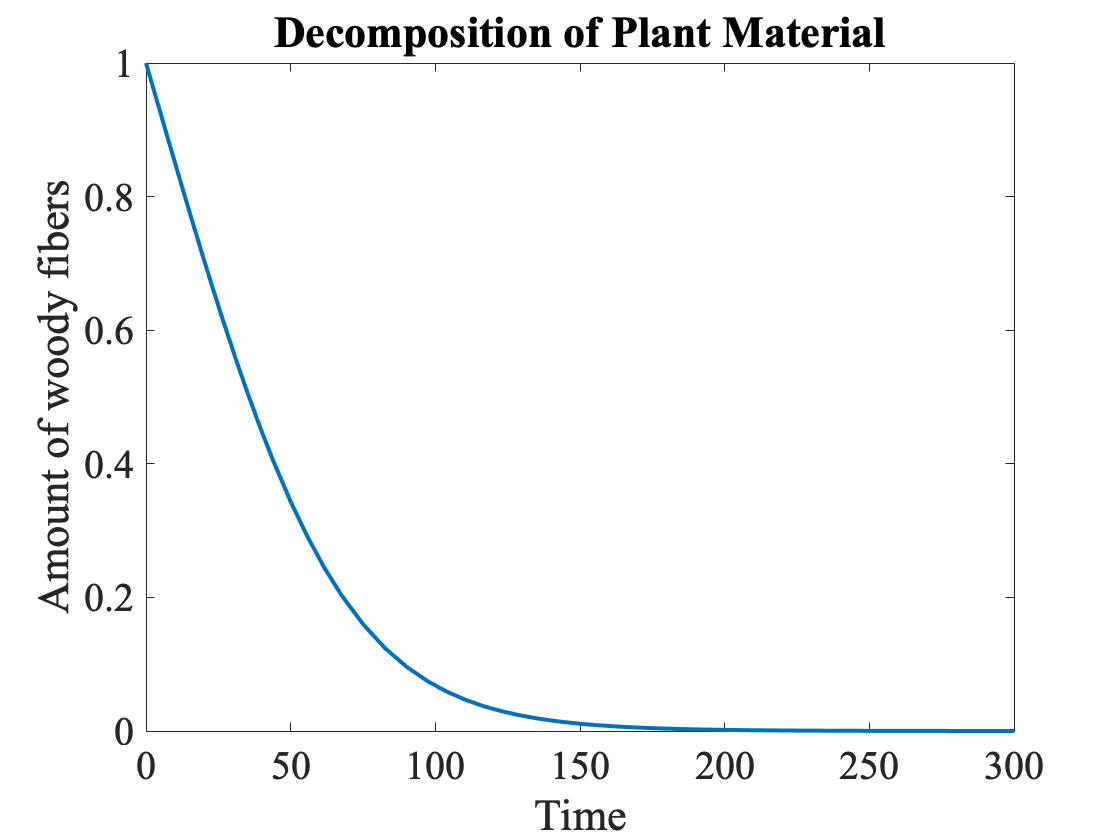
\includegraphics[width=.6\textwidth]{25_05_de.png}
	\caption{Decomposition Model}\label{fig:result}
\end{figure}
